\section{Inverse depth and estimates of scatter}
\label{section:dcmSection}
We focus on the estimation of scatter functionals of $\BF$ using peripherality-weighted sign vectors in this section. To this end, in addition to conditions (P) and (A1), we assume the following conditions on the peripherality functions:

\vspace{1em}
\noindent\textbf{(B1)} The following holds for any $\bfx \in \BR^p$ and $t \in (0,1)$:
%
$$
P(\bfx; \BF) \leq P(\bfmu_F + t(\bfx - \bfmu_F), \BF),
$$
%

\noindent\textbf{(B2)} There exists a positive constant $M(P,\BF) $ such that $P(\bfx; \BF) \rightarrow M(P,\BF)$ as $\|\bfx\| \rightarrow \infty $.
\vspace{1em}

Condition (A2) in Section~\ref{section:LocSection} is now replaced by the stronger condition (B2). Note that all the current conditions are essentially the opposite of those imposed on a traditional depth function \citep{zuo00}. Given a depth function, the peripherality functions in this section can be defined as a bounded monotonically decreasing function of it. Consequently, we use the term {\it inverse depth function} \citep{MajumdarChatterjeeStat} in place of peripherality functions in this section, denoting them by $D^-(\bfx,\BF)$, or equivalently $D^-_\bfX(\bfx)$. For ease of exposition, we stick to the following inverse transformation: $D^-_\bfX(\bfx) = \sup_\bfy D^-_\bfX(\bfy) - D^-_\bfX(\bfx)$ from now on. The theoretical results go through with minor changes for other choices of inverse depths.

Given a choice of inverse depth function $D^-_{\bfX}(\bfx)$, we transform the original random variable as: $\tilde \bfX = D^-_\bfX(\bfx) \bfS(\bfx - \bfmu)$. We use the transformed data matrix $\tilde \BX = (\tilde \bfx_1, \ldots, \tilde \bfx_n)^T$ as proxy of the original data $\BX$ for improved estimation of the components of the population covariance matrix $\Sigma$ in this section. To this end, in Section~\ref{subsec:dcm} we give some results characterizing the population covariance matrix of these vectors, i.e. $\BV \tilde \bfX$, and its affine equivariant counterpart. Section~\ref{subsec:sample-DCM} gives asymptotic properties of their finite sample versions. In Section~\ref{subsec:robustPCA}, we use eigenvectors of these estimates for robust PCA, deriving their influence functions, as well as asymptotic and finite sample efficiencies. Finally in Section~\ref{subsec:plugin}, we calculate robust estimates of eigenvalues and propose a plug-in robust estimate of $\Sigma$.

%Data depth is as much a property of a vector-valued random variable $\bfX \in \mathbb{R}^p$ as it is of the underlying distribution $F$, so for ease of notation while working with transformed random variables, from now on we shall be using $D_\bfX(\bfx) = D(\bfx, F)$ to denote the depth of a point $\bfx$. Now, given a depth function $D_{\bfX}(\bfx)$ (equivalently, an htped function $D^-_\bfX(\bfx) = D^-(\bfx, F)$), transform the original random variable as: $\tilde \bfx = \tilde D_\bfX(\bfx) \bfS(\bfx - \bfmu)$, $\bfS(.)$ being the spatial sign functional. The transformed random variable $\tilde \bfX$ can be seen as the multivariate rank corresponding to $\bfX$ (e.g. \cite{serfling2006}). 

%Figure \ref{fig:rankplot} gives an idea of how the multivariate rank vector $\tilde \bfX$ is distributed when $\bfX$ has a bivariate normal distribution. Compared to the spatial sign, which are distributed on the surface of $p$-dimensional unit ball centered at $\bfmu$, these spatial ranks have the same direction as original data and reside \textit{inside} the $p$-dimensional ball around $\bfmu$ that has radius $M_D(F)$ (which, for the case of halfspace depth, equals 0.5).

\subsection{Depth Covariance Matrix}
\label{subsec:dcm}
Consider the spectral decomposition of $\Sigma$: $\Sigma = \Gamma\Lambda\Gamma^T$, $\Gamma$ being orthogonal and $\Lambda$ diagonal with positive diagonal elements $\lambda_1 \geq \ldots \geq \lambda_p$. Also normalize the original random variable as $\bfZ = \Gamma^T\Lambda^{-1/2} (\bfX - \bfmu)$. In this setup, we can represent the transformed random variable as
%
\begin{eqnarray}
\tilde \bfX &=& D^-_{\bfX} (\bfX) \bfS(\bfX - \bfmu) \notag \\
&=& D^-_{\Gamma\Lambda^{1/2}\bfZ + \bfmu} (\Gamma\Lambda^{1/2} \bfZ + \bfmu). \bfS(\Gamma\Lambda^{1/2} \bfZ) \notag \\
&=& \Gamma D^-_{\bfZ}(\bfZ) \bfS(\Lambda^{1/2}\bfZ) \notag \\
&=& \Gamma \Lambda^{1/2} D^-_{\bfZ}(\bfZ) \bfS(\bfZ) \frac{\| \bfZ \|}{\|\Lambda^{1/2} \bfZ \|}.
\label{equation:rankdecomp}
\end{eqnarray}
%
%Because of affine (thus rotational) invariance of a depth function, the depth (htped) value at $\bfz$ does not depend on the direction of $\bfz$, i.e. $D^-_{\bfZ}(\bfz)$ and $\bfS(\bfz)$ are independent. Furthermore,
%$$ Cov \left(\bfS (\bfz), \frac{\| \bfz \|}{\|\Lambda^{1/2} \bfz\|} \right) = E \left(\bfS (\bfz). \frac{\| \bfz \|}{\|\Lambda^{1/2} \bfz\|} \right) - E \bfS (\bfz) E \left(\frac{\| \bfz \|}{\|\Lambda^{1/2} \bfz\|} \right) = E \left( \frac{\bfz}{\|\Lambda^{1/2} \bfz\|} \right) = \bf0$$
%both $\bfS (\bfz)$ and $\bfz / \| \Lambda^{1/2}\bfz \|$ are odd functions of $\bfz$, which has a circularly symmetric distribution, hence each of them has expectation $\bf0$. Consequently, we obtain an expression for the covariance matrix of $\tilde \bfX$:

$D^-_\bfZ(\cdot)$ is an even function in its argument because of affine invariance, as is $\| \bfz \| / \|\Lambda^{1/2} \bfz \|$. Since the sign function $\bfS(\cdot)$ is odd in its argument, it follows that $\BE \tilde \bfX = \bf0$. Consequently, we obtain an expression for $\tilde \Sigma := \BV \tilde \bfX$, which we call the {\it Depth Covariance Matrix} (DCM).

\begin{Theorem} \label{Theorem:covform}
Let the random variable $\bfX \in \mathbb{R}^p$ follow an elliptical distribution with center $\bfmu$ and covariance matrix $\Sigma = \Gamma\Lambda\Gamma^T$, its spectral decomposition. Then, given a depth function $D_\bfX(.)$ the covariance matrix of the transformed random variable $\tilde\bfX$ is
\begin{equation} \label{equation:covformEq1}
\tilde \Sigma = \Gamma \Lambda_{D} \Gamma^T,\quad\mbox{with}\quad \Lambda_{D} = \mathbb E_\bfZ \left[ (D^-_\bfZ(\bfz))^2 \frac{\Lambda^{1/2} \bfz \bfz^T \Lambda^{1/2}}{\bfz^T \Lambda \bfz} \right],
\end{equation}
where $\bfZ = (Z_1,...,Z_p)^T \sim N({\bf 0}, \BI_p)$, so that $\Lambda_{D}$ a diagonal matrix with diagonal entries
%
$$
\lambda_{D,i} = \mathbb E_\bfZ \left[ \frac{(D^-_\bfZ(\bfz))^2 \lambda_i z_i^2}{\sum_{j=1}^p \lambda_j z_j^2} \right].
$$
\end{Theorem}

The matrix of eigenvectors $\Gamma$ remains unchanged in the transformation $\bfX \rightarrow \tilde \bfX$. Thus the multivariate rank vectors can be used for robust principal component analysis (which we discuss shortly). However, as seen in \eqref{equation:covformEq1}, the diagonal entries of $\Lambda_{D}$ do not change if a scale change is done on all entries of $\Lambda$, meaning the $\Lambda_{D}$ matrices corresponding to $\BF$ and $c \BF$ for some $c \neq 0$ are same. Because of this reason, the DCM is not equivariant under affine transformations.

We follow the general framework of M-estimation with data-dependent weights \citep{HuberBook81} to construct an affine equivariant counterpart of the DCM. Specifically, we implicitly define the Affine-equivariant Depth Covariance Matrix (ADCM) as
%
\begin{equation} \label{eqn:ADCM}
\Sigma_{Dw} = \frac{1}{ \BV \tilde Z_1 } \BE_\bfX \left[ \frac{(D^-_\bfX(\bfx))^2 (\bfx - \bfmu) (\bfx - \bfmu)^T}{(\bfx - \bfmu)^T \Sigma_{Dw}^{-1} (\bfx - \bfmu)} \right].
\end{equation}
%
Its affine equivariance follows from the fact that the weights $(D^-_\bfX (\bfx))^2$ depend only on the standardized quantities $\bfz \sim \cE ({\bf 0}, k \bfI_p, g)$. We solve (\ref{eqn:ADCM}) iteratively by obtaining a sequence of positive definite matrices $\Sigma^{(k)}_{Dw}$ until convergence:
%
$$
\Sigma^{(k+1)}_{Dw} = \frac{1}{\BV \tilde Z_1 } \BE_\bfX \left[ \frac{(D^-_\bfX(\bfx))^2 (\Sigma^{(k)}_{Dw})^{1/2} (\bfx - \bfmu) (\bfx - \bfmu)^T (\Sigma^{(k)}_{Da})^{1/2}}{(\bfx - \bfmu)^T (\Sigma^{(k)}_{Dw})^{-1} (\bfx - \bfmu)} \right].
$$
%

To ensure existence and uniqueness of this estimator, we consider the class of scatter estimators $\Sigma_M$ that are obtained as solutions of the following equation:
%
\begin{equation}
\BE_{\bfZ_M} \left[ u( \| \bfz_M \| )  \frac{\bfz_M \bfz_M^T}{\| \bfz_M \|^2}  - v( \| \bfz_M \| ) \BI_p \right] = 0
\end{equation}
%
with $\bfz_M = \Sigma_M^{-1/2} (\bfx - \bfmu)$. Under the following assumptions on the scalar valued functions $u$ and $v$, the above equation produces a unique solution \citep{HuberBook81}:
%

\vspace{1em}
\noindent\textbf{(C1)} The function $u(r)/r^2$ is monotone decreasing, and $u(r)>0$ for $r>0$;

\noindent\textbf{(C2)}  The function $v(r)$ is monotone decreasing, and $v(r)>0$ for $r>0$;

\noindent\textbf{(C3)} Both $u(r)$ and $v(r)$ are bounded and continuous;

\noindent\textbf{(C4)} $u(0) / v(0) < p$;

\noindent\textbf{(C5)} For any hyperplane in the sample space $\mathcal X$, (i) $P(H) = \BE_\bfX \{ \BI{\bfx \in H} \} < 1 - p v(\infty) / u(\infty)$ and (ii) $P(H) \leq 1/p$.
%

\vspace{1em}
\noindent Putting things into context, in our case we have $v(r) = \BV\tilde Z_1, u(r) = (D^-_\bfX(\bfx))^2 = (D^-_\bfZ(\bfz))^2$. Since $v(r)$ is a constant, (C2) and (C3) are trivially satisfied. As for $u$, most well-known depth functions can be expressed as simple functions of the norm of the standardized random variable. For example, for Halfspace Depth (HSD) we have $D_\bfZ (\bfz) = (1 - G(\| \bfz \|)$, for Mahalanobis Depth (MhD) we have $D_\bfZ (\bfz) = (1+\| \bfz \|^2)^{-1}$ and for Projection Depth (PD) we have $D_\bfZ (\bfz) = (1+\| \bfz \|//MAD(G))^{-1}$, where $G$ is the cumulative distribution function of $g$, and MAD is median absolute deviation. Combined with the choice of inverse transformation, we get
% Var(Z1) breaks into two independent parts: depth and sign. So can check m4 and M5 here itself.
$$
u_{HSD} (r) = G^2 (r); \quad u_{MhD}(r)  = \frac{r^4}{(1 + r^2)^2}; \quad u_{PD}(r)  = \frac{r^2}{(1 + r/MAD(G))^2}.
$$
%
It is easy to verify that the above choices of $u$ satisfy (C1) and (C3). To check (C4) and (C5), notice that $\bfZ$ has a spherically symmetric distribution, so that its euclidean norm and spatial sign are independent. Since $D_\bfZ(\bfz)$ depends only on $\| \bfz \|$, we now have
%
$$
\BV \tilde Z_1 = \BV \left( D^-_\bfZ (\bfZ) \frac{Z_1}{ \|\bfZ \|} \right) = \BV (D^-_\bfZ (\bfZ)) \BV (S_1 (\bfZ)) = \frac{1}{p} \BV (D^-_\bfZ (\bfZ)),
$$
%
as $\BV(\bfS(\bfZ)) = \BV((S_1(\bfZ), S_2(\bfZ), ..., S_p(\bfZ))^T) = \BI_p/p$. Now for MhD and PD $u(\infty)=1, u(0)=0$, so (C4) and (C5) are immediate. To achieve this for HSD, we only need to replace $u_{HSD}(r)$ with $u_{HSD*}(r) = G^2(r) - 1/4$.

\subsection{Calculating the sample DCM and ADCM}
\label{subsec:sample-DCM}
Let us denote $\BS(\bfx; \bfmu) = \bfS(\bfx - \bfmu) \bfS(\bfx - \bfmu)^T$. Then, given the depth function and {\it known} location center $\bfmu$, one can show that the vectorized form of $\sqrt n$-times the sample DCM, i.e. $n^{-1/2} \sum_{i=1}^n (D^-_\bfX(\bfx_i))^2 \BS (\bfx_i; \bfmu)$  has an asymptotic multivariate normal distribution with mean $\sqrt n. \ve( \BE [( (D^-_\bfX (\bfX))^2 \BS(\bfx; \bfmu)])$ and some covariance matrix by straightforward application of the central limit theorem (CLT). But in practice the depth at any point $\bfx$ is estimated by the sample depth, i.e. depth calculated using empirical distribution function in place of $\BF$. We also need to replace the known location parameter $\bfmu$ by some estimator $\hat\bfmu_n$.

Denote this sample depth by $D^n_\bfX (\bfx)$, and the inverse depth by $D^{n-}_\bfX (\bfx)$. Here we make the following assumption regarding the sample depths:

\vspace{1em}
\noindent\textbf{(D1)} \textit{Uniform convergence}: $\sup_{\bfx \in \mathbb R^p} | D^n_\bfX (\bfx) - D_\bfX (\bfx) | \rightarrow 0$ as $n \rightarrow \infty $.
\vspace{1em}

\noindent The above holds under very mild conditions for several depth functions, e.g. projection depth \citep{zuo03} and simplicial depth \citep{Dumbgen92}. For $\hat \bfmu_n$ we use a robust estimate of location, examples of which include the spatial median \citep{haldane48,brown83}, Oja median \citep{oja83} and projection median \citep{zuo03}.

To plug in the above estimates to the sample DCM and go through with the CLT, we need the following result.

\begin{Lemma} \label{Lemma:lemma1}
Consider a random variable $\bfX \in \mathbb{R}^p$ having a continuous and symmetric distribution with location center $\bfmu$ such that $\BE \|\bfx - \bfmu \|^{-3/2} < \infty$. For a size-$n$ random sample from this distribution, suppose $\hat\bfmu_n$ is an estimator of $\bfmu$ so that $\hat\bfmu_n - \bfmu = O_P(n^{-1/2}) $. Then, given assumption (D1) we have
%
$$
\frac{1}{n} \sum_{i=1}^n (D^{n-}_\bfX (\bfx_i))^2 \BS(\bfx_i; \hat\bfmu_n) = \frac{1}{n} \sum_{i=1}^n (D^-_\bfX (\bfx_i))^2 \BS(\bfx_i; \bfmu)
+ \BR_n,
$$
%
where $\| \BR_n \|_\infty = o_P(n^{-1/2})$.
\end{Lemma}

\noindent We are now in a position to state the result for consistency of the sample DCM:

\begin{Theorem} \label{Theorem:rootn}
Consider a size-$n$ random sample from the distribution in Lemma \ref{Lemma:lemma1}. Then, given a depth function $D_\bfX(.)$ and an estimate of center $\hat\bfmu_n$ so that $\sqrt n(\hat \bfmu_n - \bfmu) = O_P(1)$,
%
$$ \ve \left\{ \frac{1}{n} \sum_{i=1}^n (D^{n-}_\bfX (\bfx_i))^2 \BS(\bfx_i; \hat\bfmu_n) \right\} -
\BE [ \ve \left\{ (D^-_\bfX (\bfx))^2 \BS(\bfx; \bfmu) \right\} ] \rightsquigarrow
\cN_{p^2} ({\bf 0}, \BV_D(\BF)) + \bfR_n,
$$
%
with $\BV_D(\BF) = \BV [\ve \{ (D^-_\bfX (\bfx))^2 \BS(\bfx; \bfmu) \} ] $ and $\| \bfR_n \|_\infty = o_P(n^{-1/2})$.
\end{Theorem}

\noindent When $\BF$ is elliptical, an elaborate form of the covariance matrix $\BV_D(\BF)$ explicitly specifying each of its elements (more directly those of its $\Gamma^T$-rotated version) can be obtained (see Appendix \ref{section:appA}). This form is useful when deriving limiting distributions of eigenvectors and eigenvalues of the sample DCM.

For ADCM, we simultaneously estimate its sample version and the mean vector $\bfmu$ by solving for the location and scatter functionals ($\bfmu_{Dw}, \Sigma_{Dw}$):
%
\begin{eqnarray}
\BE \left[ \frac{\Sigma_{Dw}^{-1/2} (\bfx - \bfmu_{Dw})}{ \| \Sigma_{Dw}^{-1/2}(\bfx - \bfmu_{Dw}) \|} \right] &=& {\bf 0}_p, \label{eqn:AffineMedian}\\
\frac{1}{\BV \tilde Z_1}
\BE \left[ \frac{(D^-_\bfX(\bfx))^2 \Sigma_{Dw}^{-1/2} (\bfx - \bfmu_{Dw}) (\bfx - \bfmu_{Dw})^T \Sigma_{Dw}^{-1/2}}{(\bfx - \bfmu_{Dw})^T \Sigma_{Dw}^{-1} (\bfx - \bfmu_{Dw})} \right] &=& \BI_p. \label{eqn:AffineCov}
\end{eqnarray}
%
In the M-estimation framework of \cite{HuberBook81}, for any fixed $\Sigma_M$ there exists a unique and fixed solution of the general location problem $\BE_{\bfZ_M} (w(\| \bfz_M \| \bfz_M) = {\bf 0}_p $ under the following condition:

\vspace{1em}
\noindent\textbf{(D2)} The function $w(r)r$ is monotone increasing for $r>0$.

\vspace{1em}
\noindent This is easy to verify for our choice of the weights: $w(\| \bfz_M \| ) = D^-_{\bfZ_M} (\bfz_M) / \| \bfz_M \|$. Uniqueness of simultaneous fixed point solutions of \eqref{eqn:AffineMedian} and \eqref{eqn:AffineCov} is guaranteed when $\bfX$ has a symmetric distribution \citep{HuberBook81}, which we also satisfy since $\bfX \sim \BF$, an elliptical distribution,

In practice, it is difficult to calculate the scale multiple $\BV \tilde Z_1$ analytically for known depth functions and an arbitrary $\BF$. We bypass this by instead obtaining a standardized version of the scatter functional: $\Sigma_{Dw}^* = \Sigma_{Dw} / \BV \tilde Z_1$ (and $\bfmu_{Dw}$) using the following iterative algorithm:

\begin{enumerate}
\item Start from some initial estimates $(\bfmu_{Dw}^{(0)}, \Sigma_{Dw}^{(0)})$. Set $t=0$;

\item Calculate the standardized observations $\bfz_i^{(t)} = (\Sigma_{Dw}^{(t)})^{-1/2} (\bfx_i - \bfmu_{Dw}^{(t)})$;

\item Update the location estimate:
%
$$
\bfmu_{Dw}^{(t+1)} = \frac{\sum_{i=1}^n \tilde \bfx_i / \| \bfz_i^{(t)} \| }{\sum_{i=1}^n \| \bfz_i^{(t)} \|^{-1} };
$$
%
\item Update the scatter estimate:
%
$$
\Sigma_{Dw}^{*(t+1)} = \frac{1}{n} \sum_{i=1}^n \frac{(D^{n-}_\bfX (\bfx_i))^2 (\bfx_i - \bfmu_{Dw}^{(t+1)})(\bfx_i - \bfmu_{Dw}^{(t+1)})^T}{\| \bfz_i^{(t)} \|^2}; \quad \Sigma_{Dw}^{*(t+1)} \leftarrow \frac{\Sigma_{Dw}^{*(t+1)}}{\text{det} (\Sigma_{Dw}^{*(t+1)})^{1/p}}.
$$
%
\item Continue until convergence.
\end{enumerate}

\subsection{Robust PCA using eigenvectors}
\label{subsec:robustPCA}
We are mainly interested in using the DCM for robust principal component analysis (PCA). We assume that the eigenvalues of $\Sigma$ are distinct: $\lambda_1 > \lambda_2 > ... > \lambda_p$, for ease of obtaining asymptotic distributions of eigenvectors of the DCM (Appendix \ref{section:appB}). Limiting distributions for the case of non-unique eigenvalues can be obtained following \cite{magyar14}.

\subsubsection{Influence functions}
To demonstrate the robustness of eigenvector estimates of the DCM and ADCM, we derive their influence functions. Influence functions quantify how much influence a sample point, especially an infinitesimal contamination, has on any functional of a probability distribution \citep{HampelBook86}. Given any probability distribution $\BH \in \cM$, the influence function of any point $\bfx_0 \in \mathcal{X}$ for some functional $T(\BH)$ on the distribution is defined as
%
$$
IF(\bfx_0; T,\BH) =
\lim_{\epsilon \rightarrow 0} \frac{1}{\epsilon} (T(\BH_\epsilon) - T(\BH))
$$
%
where $\BH_\epsilon$ is $\BH$ with an additional mass of $\epsilon$ at $\bfx_0$, i.e. $\BH_\epsilon = (1-\epsilon)\BH + \epsilon \Delta_{\bfx_0}$; $\Delta_{\bfx_0}$ being the distribution with point mass at $\bfx_0$. When $T(\BH) = E_\BH f$ for some $\BH$-integrable function $f$, $IF(\bfx_0; T,\BH) = f(\bfx_0) - T(\BH)$.

It now follows that for the DCM,
%
$$
IF(\bfx_0; \tilde \Sigma, \BF) =
(D^-_\bfX(\bfx_0))^2 \BS(\bfx_0; \bfmu) - \tilde \Sigma.
$$
%
Following \cite{croux00}, we get the influence function of the $i^\text{th}$ eigenvector of $\tilde \Sigma$, say $\bfgamma_D = (\gamma_{D,1},...,\gamma_{D,p})^T$ for $1 \leq i \leq p$:
%
\begin{eqnarray}
IF(\bfx_0; \bfgamma_{D,i}, \BF) &=&
\sum_{k=1; k \neq i}^p \frac{1}{\lambda_{D,i} - \lambda_{D,k}} \left\{ \bfgamma^T_k IF(\bfx_0; \tilde \Sigma, \bfgamma_i) \right\} \bfgamma_k \notag \\
&=& \sum_{k=1; k \neq i}^p \frac{1}{\lambda_{D,i} - \lambda_{D,k}}
\left\{ \bfgamma^T_k (D^-_\bfX(\bfx_0))^2 \BS(\bfx_0; \bfmu)\bfgamma_i - \lambda_{D,i}\bfgamma_k^T\bfgamma_i \right\} \bfgamma_k \notag \\
&=& \sum_{k=1; k \neq i}^p \frac{\sqrt{\lambda_i \lambda_k} z_{0i} z_{0k}}{\lambda_{D,i} - \lambda_{D,k}}. \frac{(D^-_\bfZ(\bfz_0))^2 }{\bfz_0^T \Lambda \bfz_0} \bfgamma_k \notag\\
&=& \sum_{k=1; k \neq i}^p \frac{(D^-_\bfZ(\bfz_0))^2 \BS_{ik}(\Lambda^{1/2} \bfz_0; {\bf 0})}{\lambda_{D,i} - \lambda_{D,k}} \bfgamma_k,
\end{eqnarray}
%
where $\Gamma^T \Lambda^{-1/2} (\bfx_0 - \bfmu) = \bfz_0 = (z_{01},...,z_{0p})^T$. Clearly this influence function is bounded, indicating good robustness properties of the principal component estimates.

\begin{figure}[]
	\centering
		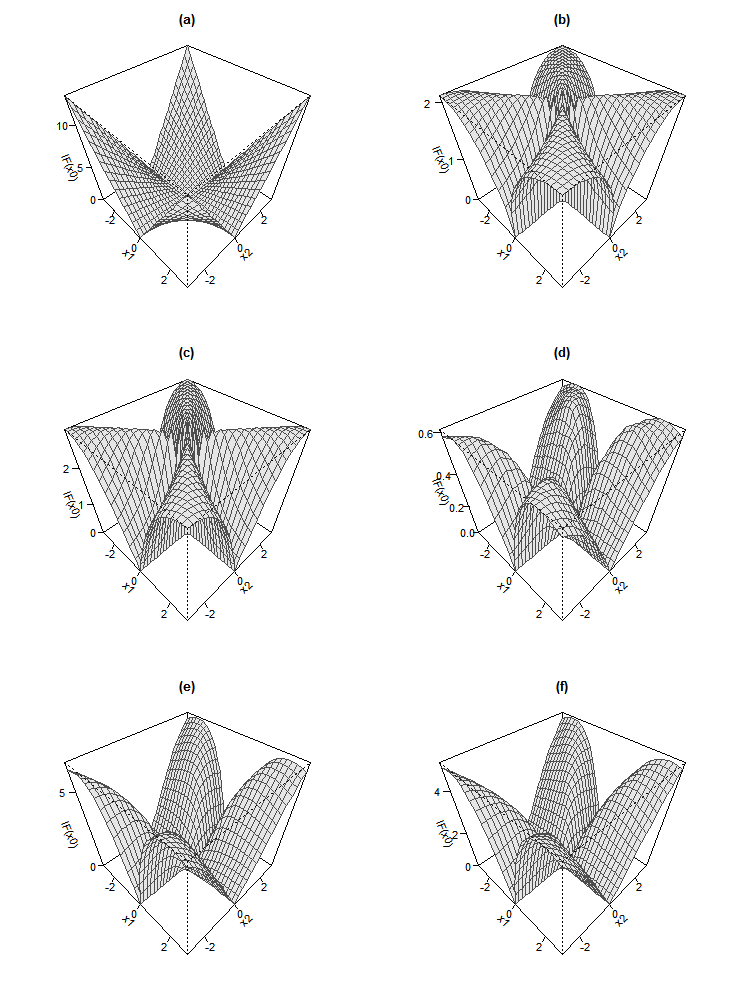
\includegraphics[width=12cm]{../Codes/IFnorm.png}
	\caption{Plot of the norm of influence function for first eigenvector of (a) sample covariance matrix, (b) SCM, (c) Tyler's scatter matrix and DCMs for (d) Halfspace depth, (e) Mahalanobis depth, (f) Projection depth for a bivariate normal distribution with $\bfmu = {\bf 0}, \Sigma = \diag(2,1)$}
	\label{fig:IFnorm}
\end{figure}

In Figure \ref{fig:IFnorm} we consider first eigenvectors of the DCM and two other well-known robust estimates of scatter: the Sign Covariance Matrix (SCM) and Tyler's shape matrix \citep{tyler87}. We set $\BF \equiv \mathcal{N}_2({\bf 0}, \diag(2,1))$ and plot norms of the eigenvector influence functions for different values of $\bfx_0$. Influence function for the $i^\text{th}$ eigenvectors of these two matrices (say $\bfgamma_{S,i}$ and $\bfgamma_{T,i}$, respectively) are as follows:
%
\begin{eqnarray}
\quad IF(\bfx_0; \bfgamma_{S,i}, \BF) &=&
\sum_{k=1; k \neq i}^p \frac{\BS_{ik}(\Lambda^{1/2} \bfz_0, {\bf 0})}{\lambda_{S,i} - \lambda_{S,k}} \bfgamma_k; \quad
\lambda_{S,i} = \BE_\bfZ \left( \frac{\lambda_i z_i^2}{\sum_{j=1}^p \lambda_j z_j^2} \right),\\
IF(\bfx_0; \bfgamma_{T,i}, \BF) &=& (p+2) \sum_{k=1; k \neq i}^p \frac{\sqrt{\lambda_i \lambda_k}}{\lambda_i - \lambda_k}\BS_{ik}(\bfz_0; {\bf 0}) \bfgamma_k. \label{eqn:IFeqnTyler}
\end{eqnarray}
%
Their corresponding plots (panels (b) and (c) in Figure~\ref{fig:IFnorm}) demonstrate an `inlier effect', i.e. points close to symmetry center and the center itself having high influence: which results in loss of efficiency. The influence function for eigenvector estimates of the sample covariance matrix is obtained by replacing $(p+2)$ by $\| \bfz_0 \|^2$ in \eqref{eqn:IFeqnTyler}, hence is unbounded and makes the corresponding estimates non-robust. In comparison, all three DCMs considered have bounded influence functions {\it and} small values of the influence function at `deep' points.

For the ADCM, we first notice that the influence function of any affine equivariant estimate of scatter can be expressed as
%
$$
IF(\bfx_0, C, \BF) = \alpha_C (\| \bfz_0 \| ) \BS(\bfz_0; {\bf 0}) - \beta_C( \| \bfz_0 \| ) C
$$
%
for scalar valued functions $\alpha_C, \beta_C$ \citep{HampelBook86}. Following this, the influence function of an eigenvector $\bfgamma_{C,i}$ of $C$ is derived:
%
$$
IF(\bfx_0, \bfgamma_{C,i}, \BF) = \alpha_C(\| \bfz_0 \|) \sum_{k=1, k \neq i}^p \frac{\sqrt {\lambda_i \lambda_k}}{\lambda_i - \lambda_k}. \BS_{ik}(\bfz_0; {\bf 0}) \bfgamma_k.
$$
%
When $C=\Sigma_M$, i.e. the solution to (\ref{eqn:ADCM}), \cite{HuberBook81} shows that
%
$$
\alpha_C (\| \bfz_0 \|) = \frac{p(p+2) u (\| \bfz_0 \|)}{\BE_{\bfZ} \left[ p u(\| \bfz \| ) + u'(\| \bfz \|) \| \bfz \| \right] }.
$$
%
In our case $u( \| \bfz_0 \|) = ( D^-_\bfZ (\bfz_0))^2$, thus the influence function of eigenvectors of the ADCM is a bounded increasing function of $\| \bfz_0 \|$.

\subsubsection{Asymptotic and finite-sample efficiencies}

%Unlike affine equivariant estimators of shape, the Asymptotic Relative Efficiency (ARE) of eigenvectors (with respect to any other affine equivariant estimator) can not be simplified as a ratio of two scalar quantities dependent on only the distribution of $\| \bfz \|$ (e.g. \cite{taskinen12,ollilia03}).
The asymptotic variance of the $i\Th$ eigenvector of the sample covariance matrix, say $\hat \bfgamma_i$, is \citep{anderson}:
%
\begin{equation} \label{equation:covevEq}
A\BV( \sqrt n\hat \bfgamma_{i}) = \sum_{k=1; k \neq i}^p \frac{\lambda_i \lambda_k}{(\lambda_i - \lambda_k)^2} \bfgamma_k \bfgamma_k^T; \quad
1 \leq i \leq p.
\end{equation}
%
Asymptotic relative efficiencies of eigenvectors from the sample DCM with respect to the sample covariance matrix can now be derived using (\ref{equation:covevEq}) and (\ref{equation:DevEq}) from Corollary \ref{Corollary:eigendist} from Appendix \ref{section:appB}:
%
\begin{eqnarray*}
ARE(\hat\bfgamma_{D,i}, \hat\bfgamma_i; \BF) &=& \frac{\Tr( A\BV ( \sqrt n\hat \bfgamma_i))}{\Tr( A\BV(\sqrt n\hat \bfgamma_{D,i}))}\\
&=& \left[\sum_{k=1; k \neq i}^p \frac{\lambda_i \lambda_k}{(\lambda_i - \lambda_k)^2} \right] \left[ \sum_{k=1; k \neq i}^p
\frac{\BE [ (D^-_\bfZ (\bfz))^4 (\BS_{ik} (\Lambda^{1/2} \bfz; {\bf 0}))^2 ]}{(\lambda_{D,i} - \lambda_{D,k})^2} \right]^{-1}.
\end{eqnarray*}

Obtaining ARE of the ADCM is, in comparison to DCM, more straightforward. The asymptotic covariance matrix of an eigenvector of the affine equivariant scatter functional $C$ is given by:
%
$$
A\BV (\sqrt n  \hat\bfgamma_{C,j}) = A\BV (C_{12}, \BF_0) \sum_{k=1, k \neq i}^p \frac{\lambda_i \lambda_k}{\lambda_i - \lambda_k}. \bfgamma_i \bfgamma_k^T,
$$
%
where $A\BV (C_{12}, \BF_0)$ is the asymptotic variance of an off-diagonal element of $C$ when the underlying distribution is $\BF_0 \equiv \cE({\bf 0}, \BI_p, g)$. Following \cite{croux00} this equals
%
$$
A\BV (C_{12}, \BF_0) = \BE_{\bfZ} \left[ (\alpha_C (\| \bfz \|) \BS_{12} (\bfz; {\bf 0}))^2 \right] = \BE_{\bfZ} \alpha_C (\| \bfz \|)^2 . \BE_{\bfZ} (\BS_{12}(\bfz; {\bf 0}))^2,
$$
% 
using the fact that $\|\bfZ\|$ and $\bfS(\bfZ)$ are independent with $\bfZ \sim \BF_0$. It now follows that
%
\begin{equation}
ARE (\hat\bfgamma_{\Sigma_M,i}, \hat\bfgamma_{i}; \BF) =
\frac{1}{A\BV (C_{12}, \BF_0)} = \frac{\left[ \BE_{\bfZ} ( p u \| \bfz\| + u'( \| \bfz \|) \| \bfz \| ) \right]^2}
{p^2 (p+2)^2 \BE_\bfZ (u (\| \bfz \|)^2 \BE_{\bfZ} (\BS_{12}(\bfz; {\bf 0}))^2}.
\end{equation}
%

Table \ref{table:AREtable} considers 6 different elliptic distributions (namely, $p$-variate $t$ with df = 5, 6, 10, 15, 25 and multivariate normal) and summarizes ARE of the first eigenvectors for ADCMs corresponding to projection depth (PD-ACM) and halfspace depth (HSD-ACM). Due to difficulty in analytically obtaining the AREs, we calculate them using Monte-Carlo simulation of $10^6$ samples and subsequent numerical integration. The ADCM seems to be particularly efficient in lower dimensions for distributions with heavier tails ($t_5$ and $t_6$), while for distributions with lighter tails, the AREs increase with data dimension. At higher values of $p$ the ADCM is almost as efficient as the sample covarnace matrix when the data comes from multivariate normal distribution.

\begin{table}[t]
\centering
\begin{footnotesize}
\begin{tabular}{c|cccc|cccc}
    \hline
    & \multicolumn{4}{c|}{PD-ACM} & \multicolumn{4}{c}{HSD-ACM} \\\cline{2-9}
    Distribution & $p=2$  & $p=5$  & $p=10$ & $p=20$ & $p=2$  & $p=5$  & $p=10$ & $p=20$ \\ \hline
    $t_5$           & 4.73 & 3.99 & 3.46 & 3.26 & 4.18 & 3.63 & 3.36 & 3.15 \\
    $t_6$           & 2.97 & 3.28 & 2.49 & 2.36 & 2.59 & 2.45 & 2.37 & 2.32 \\
    $t_{10}$          & 1.45 & 1.47 & 1.49 & 1.52 & 1.30 & 1.37 & 1.43 & 1.49 \\
    $t_{15}$          & 1.15 & 1.19 & 1.23 & 1.27 & 1.01 & 1.10 & 1.17 & 1.24 \\
    $t_{25}$          & 0.97 & 1.02 & 1.07 & 1.11 & 0.85 & 0.94 & 1.02 & 1.08 \\
    MVN          & 0.77 & 0.84 & 0.89 & 0.93 & 0.68 & 0.77 & 0.84 & 0.91 \\ \hline
\end{tabular}
\end{footnotesize}
\caption{Table of AREs of the ADCM for different choices of $p$ and data-generating distributions, and two choices of depth functions}
\label{table:AREtable}
\end{table}

We also obtain finite sample efficiencies of the three DCMs and ADCMs by a simulation study for $p=4$, and compare them with the same from the SCM and Tyler's scatter matrix. We consider the same 6 elliptical distributions considered in ARE calculations above, and from every distribution draw 10000 samples each for sample sizes $n = 20, 50, 100, 300, 500$. All distributions are centered at ${\bf 0}_p$, and have covariance matrix $\Sigma = \diag(4,3,2,1)$.

We use the concept of principal angles \citep{miao92} to find out error estimates for the first eigenvector of a scatter matrix. In our case, the first eigenvector is
%
$$
\bfgamma_1 = (1,\overbrace{0,...,0}^{p-1})^T.
$$
%
We measure the prediction error for an eigenvector estimate by some method, say $\hat\bfgamma_{E,1}$, by the smallest angle between the true and predicted vectors, i.e. $ \cos^{-1} | \hat\bfgamma_{E,1}^T \hat\bfgamma_1 | $. A small absolute value of this angle means to better prediction. We repeat this 10000 times and calculate the \textbf{Mean Squared Prediction Angle}:
%
$$
MSPA(\hat \bfgamma_{E,1}) =
\frac{1}{10000} \sum_{m=1}^{10000} \left( \cos^{-1} \left|\bfgamma_1^T \hat\bfgamma^{(m)}_{E,1} \right| \right)^2.
$$
%
The finite sample efficiency of this eigenvector estimate relative to that from the sample covariance matrix, i.e. $\hat\bfgamma_1$ is obtained as:
$$ FSE(\hat\bfgamma_{E,1}, \hat\bfgamma_1) = \frac{MSPA(\hat\bfgamma_1)}{MSPA(\hat\bfgamma_{E,1})}.$$

As seen in Table~\ref{table:FSEtable4} for $p = 4$, DCM- and ADCM-based estimators (columns 3-5) outperform SCM and Tyler's M-estimate of scatter. Among the 3 depth functions considered, projection depth gives the best results. Its finite sample performances are better than Tyler's and Huber's M-estimators of scatter, as well as their symmetrized counterparts that are much more computationally intensive (see Table 4 in \cite{sirkia07}). The affine equivariant versions of all DCMs (columns 6-8) further improve their performance.

\begin{table}[t]
\begin{scriptsize}
    \begin{tabular}{c|cc|ccc|ccc}
    \hline
    4-variate $t_5$    & SCM  & Tyler & DCM-H & DCM-M & DCM-P & ADCM-H & ADCM-M & ADCM-P \\ \hline
    $n$=20             & 1.04 & 1.02  & 1.10   & 1.07   & 1.02  & 1.09    & 1.07    & 0.98   \\
    $n$=50             & 1.08 & 1.08  & 1.16   & 1.16   & 1.13  & 1.19    & 1.19    & 1.13   \\
    $n$=100            & 1.31 & 1.31  & 1.42   & 1.38   & 1.36  & 1.46    & 1.44    & 1.36   \\
    $n$=300            & 1.46 & 1.54  & 1.81   & 1.76   & 1.95  & 1.88    & 1.88    & 1.95   \\
    $n$=500            & 1.92 & 1.93  & 2.23   & 2.03   & 2.31  & 2.35    & 2.19    & 2.39   \\ \hline
    4-variate $t_6$    & SCM  & Tyler & DCM-H & DCM-M & DCM-P & ADCM-H & ADCM-M & ADCM-P \\ \hline
    $n$=20             & 1.00 & 1.05  & 1.03   & 1.05   & 1.00  & 1.04    & 1.04    & 0.95   \\
    $n$=50             & 1.03 & 1.01  & 1.13   & 1.12   & 1.11  & 1.19    & 1.17    & 1.10   \\
    $n$=100            & 1.08 & 1.12  & 1.25   & 1.23   & 1.27  & 1.24    & 1.25    & 1.22   \\
    $n$=300            & 1.34 & 1.36  & 1.64   & 1.52   & 1.60  & 1.67    & 1.61    & 1.68   \\
    $n$=500            & 1.26 & 1.34  & 1.55   & 1.49   & 1.60  & 1.65    & 1.61    & 1.69   \\ \hline
    4-variate $t_{10}$ & SCM  & Tyler & DCM-H & DCM-M & DCM-P & ADCM-H & ADCM-M & ADCM-P \\ \hline
    $n$=20             & 0.90 & 0.89  & 0.95   & 0.98   & 0.98  & 0.96    & 1.01    & 0.95   \\
    $n$=50             & 0.90 & 0.91  & 1.01   & 0.98   & 0.98  & 1.03    & 1.04    & 0.99   \\
    $n$=100            & 0.87 & 0.87  & 0.93   & 0.95   & 1.01  & 0.99    & 1.01    & 1.05   \\
    $n$=300            & 0.87 & 0.87  & 1.09   & 1.09   & 1.17  & 1.14    & 1.16    & 1.23   \\
    $n$=500            & 0.88 & 0.92  & 1.10   & 1.10   & 1.23  & 1.19    & 1.22    & 1.29   \\ \hline
    4-variate $t_{15}$ & SCM  & Tyler & DCM-H & DCM-M & DCM-P & ADCM-H & ADCM-M & ADCM-P \\ \hline
    $n$=20             & 0.92 & 0.90  & 0.94   & 0.94   & 0.96  & 0.95    & 0.97    & 0.89   \\
    $n$=50             & 0.82 & 0.83  & 0.88   & 0.91   & 0.93  & 0.88    & 0.93    & 0.93   \\
    $n$=100            & 0.84 & 0.87  & 0.92   & 0.95   & 1.00  & 0.93    & 0.96    & 1.00   \\
    $n$=300            & 0.73 & 0.75  & 0.96   & 0.99   & 1.10  & 1.00    & 1.06    & 1.12   \\
    $n$=500            & 0.73 & 0.76  & 0.95   & 0.96   & 1.06  & 0.94    & 0.97    & 1.06   \\ \hline
    4-variate $t_{25}$ & SCM  & Tyler & DCM-H & DCM-M & DCM-P & ADCM-H & ADCM-M & ADCM-P \\ \hline
    $n$=20             & 0.89 & 0.92  & 0.92   & 0.92   & 0.90  & 0.96    & 0.95    & 0.89   \\
    $n$=50             & 0.82 & 0.84  & 0.89   & 0.90   & 0.91  & 0.93    & 0.96    & 0.92   \\
    $n$=100            & 0.77 & 0.76  & 0.90   & 0.90   & 0.96  & 0.94    & 0.98    & 1.04   \\
    $n$=300            & 0.73 & 0.77  & 0.93   & 0.91   & 0.98  & 1.00    & 0.98    & 1.03   \\
    $n$=500            & 0.67 & 0.71  & 0.83   & 0.83   & 0.96  & 0.88    & 0.90    & 1.00   \\ \hline
    4-variate Normal   & SCM  & Tyler & DCM-H & DCM-M & DCM-P & ADCM-H & ADCM-M & ADCM-P \\ \hline
    $n$=20             & 0.82 & 0.84  & 0.87   & 0.90   & 0.91  & 0.89    & 0.93    & 0.89   \\
    $n$=50             & 0.80 & 0.81  & 0.87   & 0.88   & 0.88  & 0.88    & 0.92    & 0.88   \\
    $n$=100            & 0.68 & 0.71  & 0.80   & 0.85   & 0.91  & 0.82    & 0.86    & 0.92   \\
    $n$=300            & 0.61 & 0.63  & 0.82   & 0.85   & 0.93  & 0.86    & 0.91    & 0.96   \\
    $n$=500            & 0.60 & 0.64  & 0.77   & 0.80   & 0.90  & 0.82    & 0.86    & 0.96   \\ \hline
    \end{tabular}
\end{scriptsize}
\caption{Finite sample efficiencies of several scatter matrices: $p=4$. H, M or P after DCM or ADCM indicates the depth function used: H = halfspace depth, M = Mahalanobis depth, P = projection depth.}
\label{table:FSEtable4}
\end{table}

\subsection{Robust estimation of eigenvalues, and a plug-in estimator of $\Sigma$}
\label{subsec:plugin}
As seen in Theorem~\ref{Theorem:covform}, eigenvalues of the DCM are not same as the population eigenvalues, whereas the ADCM only gives back standardized eigenvalues. However, it is possible to robustly estimate the original eigenvalues by working with the individual columns of the robust score matrix. We do so using the following steps:

\begin{enumerate}
\item Randomly divide the sample indices $\{1,2,...,n\}$ into $k$ disjoint groups $\{G_1,...,G_k \}$ of size $\lfloor n/k \rfloor$ each;

\item Assume the data is centered. Transform the data matrix: $\BS = \hat\Gamma^T_D \BX$;

\item Calculate coordinate-wise variances for each group of indices $G_j$:
%
$$
\hat\lambda_{i,j} = \frac{1}{|G_j|} \sum_{l \in G_j} (s_{li} - \bar s_{G_j,i})^2; \quad i = 1,...,p; j = 1,...,k
$$
where $\bar\bfs_{G_j} = (\bar s_{G_j,1}, ..., \bar s_{G_j,p})^T$ is the vector of column-wise means of $\BS_{G_j}$, the submatrix of $\BS$ with row indices in $G_j$.
%
\item Obtain estimates of eigenvalues by taking coordinate-wise medians of these variances:
%
$$
\hat \lambda_i = \text{median} (\hat\lambda_{i,1}, ... , \hat\lambda_{i,k} ); \quad i = 1,...,p
$$
%
\end{enumerate}
%
The number of subgroups used to calculate this median-of-small-variances estimator can be determined following \cite{Minsker15}. After this, we construct a consistent plug-in estimator of the population covariance matrix $\Sigma$:

\begin{Theorem}\label{Thm:pluginSigma}
Consider the estimates $\hat\lambda_i$ obtained from the above algorithm, and the matrix of eigenvectors $\hat\Gamma_D$ estimated using the sample DCM. Define $\hat\Sigma = \hat\Gamma_D \hat\Lambda \hat\Gamma_D^T; \hat\Lambda = \diag(\hat\lambda_1, ..., \hat\lambda_p)$. Then as $n \rightarrow \infty$,
%
$$
\| \hat\Sigma - \Sigma \|_F \stackrel{P}{\rightarrow} 0.
$$
%
\end{Theorem}

%{\colrbf (put in 1 or 2 sentences?)}
